\nsection{OSN 12 Методы контроля качества ПО. Верификация и валидация. Виды верификации. Экспертиза. Статический и динамический анализ. Формальные методы верификации. Проверка моделей.}

\textbf{Методы контроля качества ПО} предназначены для проверки различных характеристик качества ПО и поиска различных дефектов, связанных с недостаточным качеством. Они обычно разделяются на верификацию и валидацию. Они обычно разделяются на верификацию и валидацию.

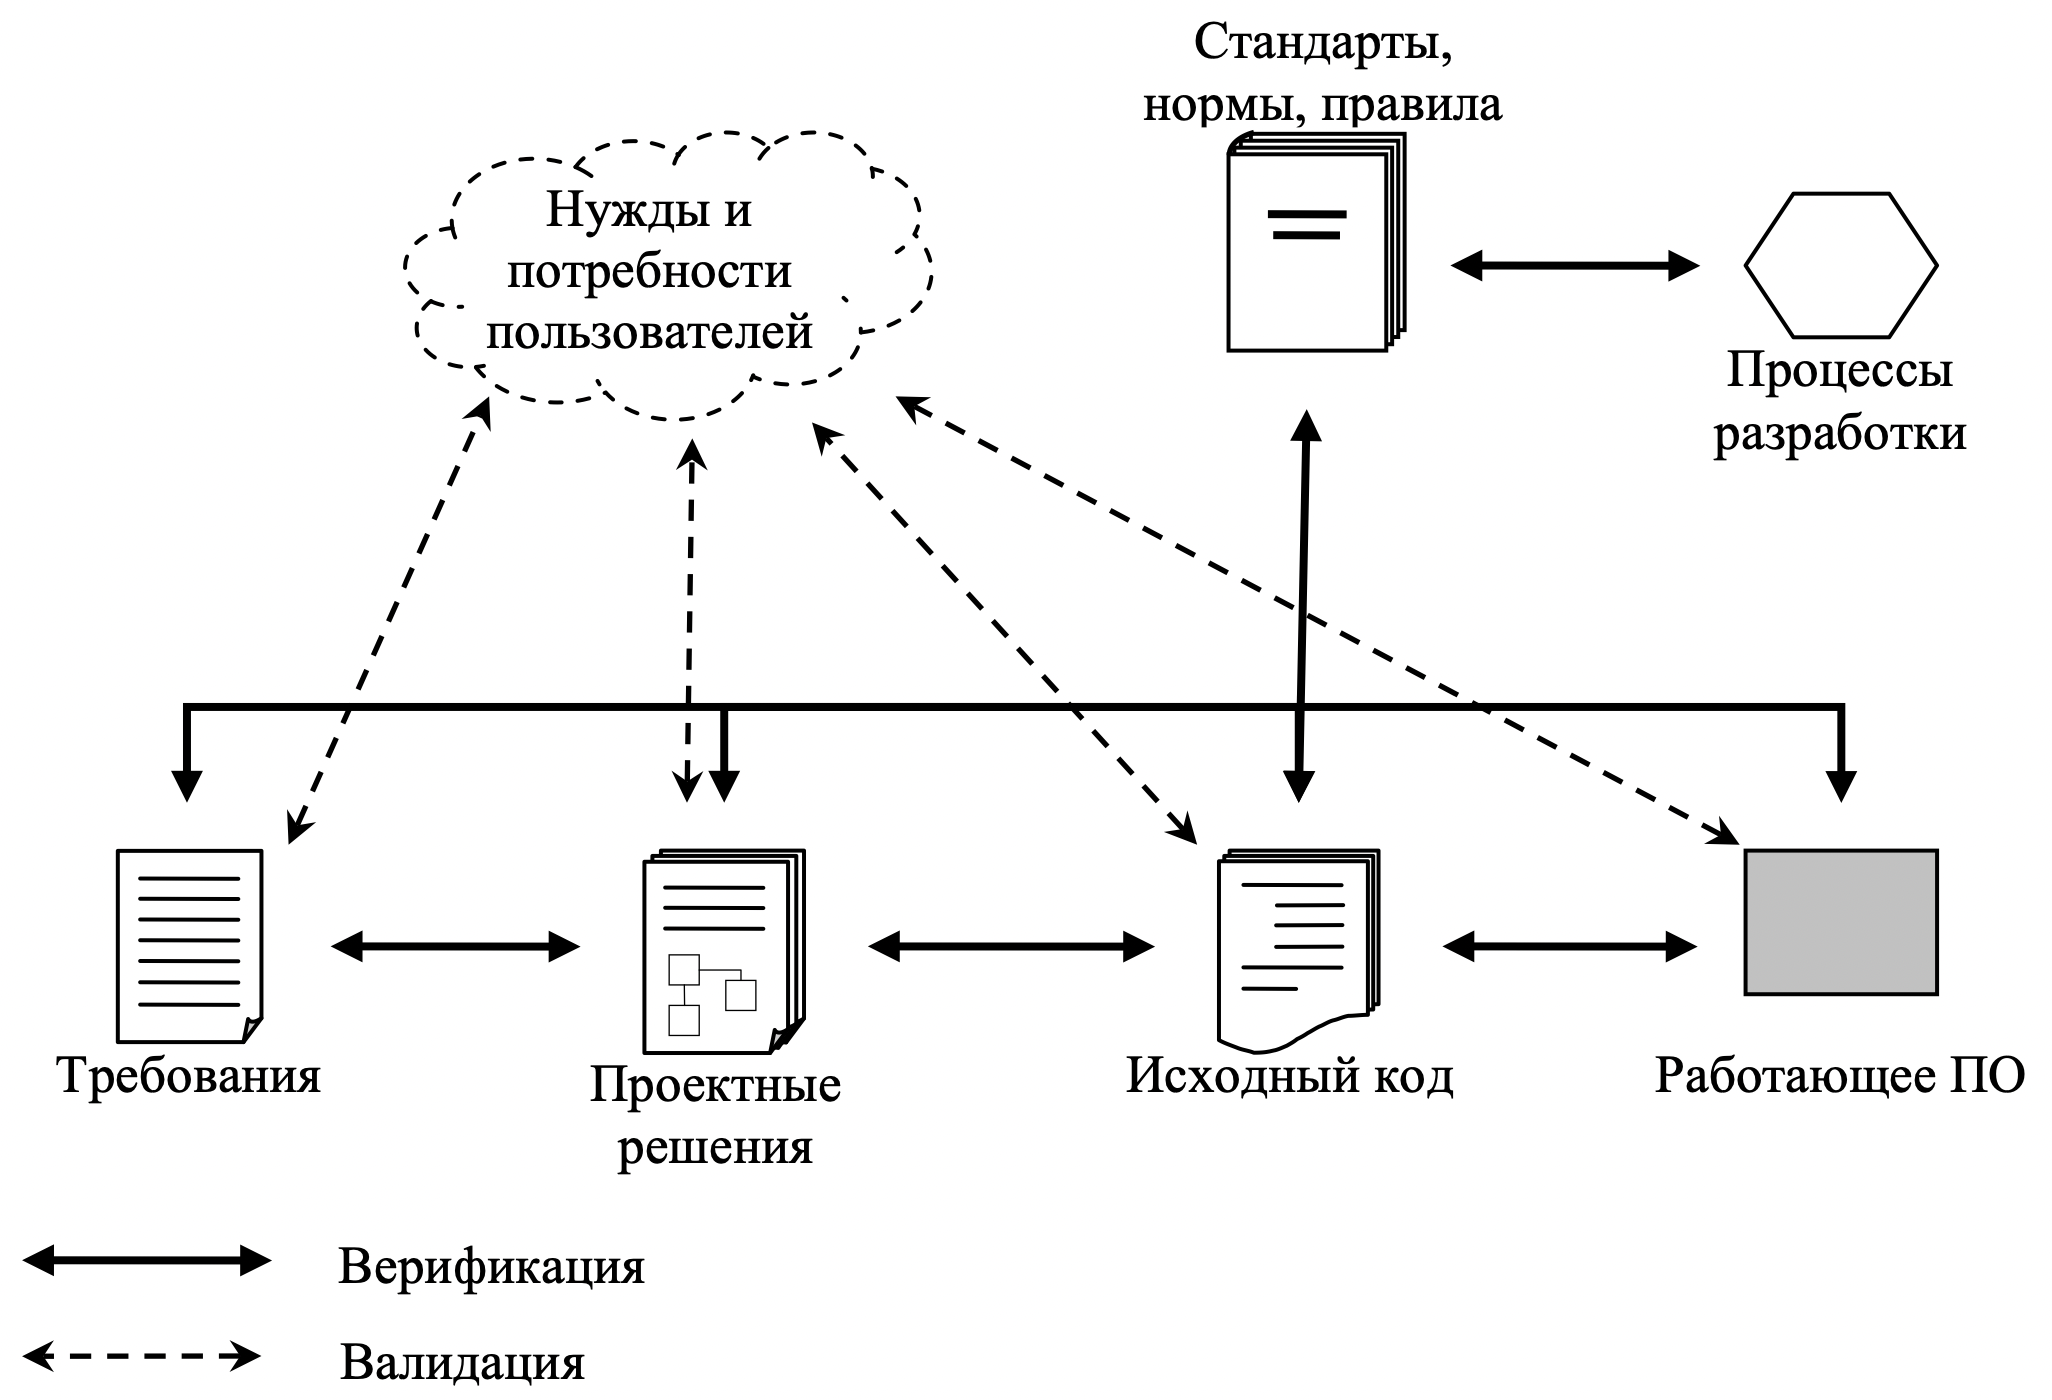
\includegraphics[scale=0.27]{pics/12_01.png}

\textbf{Валидация} обозначает проверку некоторого артефакта разработки на соответствие конечным целям, для достижения которых это ПО предназначено, т. е., нуждам и потребностям его пользователей и заказчиков. При валидации ПО проверяется, что оно действительно решает нужные пользователям задачи и удовлетворяет их потребности (даже если эти задачи и потребности описаны плохо и неполно). Валидация обычно проводится представителями заказчика, пользователями, экспертами в предметной области, т.е. людьми, обладающими достаточной компетентностью, чтобы судить о достижении поставленных целей. Если же эти цели формализовать, описать точно и полно, то проверка на соответствие полученному документу будет верификацией. Валидация необходима, потому что обычно согласованное, полное и точное описание задач сложной системы практически невозможно, разрабатываемые документы со спецификациями требований и пр. являются только приближениями к такому описанию. При валидации, могут использоваться те же техники, что и при выявления требований, поскольку цели этих видов деятельности похожи — преобразовать неясные и неформальные пожелания и представления о работе ПО в более точную форму (при валидации — в оценку проверяемых характеристик качества).

В рамках \textbf{верификации} качество некоторого артефакта (документа, модели, элемента кода и пр.) проверяется за счет сопоставления его с другим артефактом, на основе которого первый должен был быть разработан или которому он должен соответствовать (а также за счет проверки его соответсвия принятым нормам и стандартам разработки). Так, верифицировать код можно, имея на руках описание требований, проектные решения или стандарты кодирования, верифицировать проектный документ можно с помощью требований или стандартов на оформление подобных документов. Верифицировать можно и реальное поведение системы — сопоставляя его с требованиями, проектными решениями, принятыми стандартами функционирования систем такого рода. Методы верификации делятся на следующие группы:

\underline{\textit{1. Методы экспертизы}}. При экспертизе верификацию проводит человек, обладающий значительным опытом проведения такого рода проверок (часто также в экспертизу включаются неопытные сотрудники с целью их обучения). Экспертиза бывает общей, нацеленной на выявление любых дефектов и ошибок, или специализированной, направленной на оценку отдельных характеристик качества (например, гибкости архитектуры, удобства использования или защищенности ПО). Обычно в качестве видов экспертиз выделяют организационные экспертизы, технические экспертизы, сквозной контроль, инспекции и аудиты. Экспертиза применима к любым свойствам ПО и любым артефактам жизненного цикла и на любом этапе проекта, хотя для разных целей могут использоваться разные ее виды. Она позволяет выявлять практически любые виды ошибок, причем делать это на этапе подготовки соответствующего артефакта, тем самым минимизируя время существования дефекта и его последствия для качества итогового продукта. В то же время экспертиза весьма трудоемка, требует активного участия опытных людей и не может быть автоматизирована. Эффективность экспертизы существенно зависит от опыта и мотивации ее участников, организации процесса, а также от обеспечения корректного взаимодействия между различными участниками. Это накладывает дополнительные ограничения на распределение ресурсов в проекте и может приводить к конфликтам между разработчиками, если руководство проекта обращает мало внимания на коммуникативные аспекты проведения экспертиз.

\underline{\textit{2. Статический анализ}}. Такие методы используют автоматический анализ кода, моделей или других документов разработки с целью проверки выполнения формализованных правил их оформления (синтаксической корректности) и поиска часто встречающихся ошибок по определенным шаблонам (разыменования нулевых указателей, обращения к неинициализированным данным, деления на 0, взаимной блокировки параллельных процессов и пр.).
Статический анализ выполняется с помощью специализированных инструментов, техники статического анализа кода, которые достигли достаточной зрелости и поддерживаются эффективными алгоритмами, чаще всего включаются в состав компиляторов. Однако, статический анализ обычно способен выявлять лишь ограниченный набор видов ошибок.
Основной проблемой многих техник статического анализа является следующая дилемма: либо используются строгие методы анализа, не допускающие пропуска ошибок (тех типов, что ищутся), но приводящие к большому количеству сообщений о возможных ошибках, которые таковыми не являются (ложные сообщения об ошибках), либо набор сообщений об ошибках является точным, но возникает возможность пропустить ошибку. Обычно используются компромиссные решения, позволяющие обнаруживатькак можно больше ошибок, но допускающие не слишком высокий процент ложных сообщений.

\underline{\textit{3. Динамический анализ}}. Эти методы выполняют верификацию реальной работы ПО или работы его кода или исполнимой модели (из которой код получают автоматизированной трансляцией) в специализированном окружении (например, при отсутствии нужного оборудования или внешних систем производится их эмуляция). При этом собирается информация о результатах работы в различных ситуациях, и эта информация далее подвергается анализу на предмет соответсвия требованиям или проектным решениям. Обычно к таким методам относят тестирование, при котором работа ПО проверяется на заранее выбранном наборе ситуаций; мониторинг, в рамках которого работа ПО протоколируется и оценивается при его обычной или пробной эксплуатации; а также профилирование, специфический вид мониторинга временных характеристики работы ПО и использования им отдельных ресурсов. К динамическим методам анализа относят также и имитационное тестирование и имитационный мониторинг, при которых ПО выполняется в рамках какого-то модельного окружения, построенного с использованием симуляторов и эмуляторов. Для применения динамических методов необходимо иметь работающую систему или хотя бы некоторые ее компоненты, или же их прототипы, поэтому нельзя использовать их на первых стадиях разработки.

\underline{\textit{4. Формальные методы верификации}} используют формальные математические модели проверяемого артефакта и того, на соответствие которому проводится проверка. Чаще всего это модели, соответственно, кода или проектных решений и требований. К формальным методам относятся дедуктивный анализ и проверка моделей. В рамках дедуктивного анализа свойства кода или проектных решений, а также требования формализуются в виде наборов логических утверждений (могущих включать элементы логики высших порядков и различных алгебраических структур), и из первого набора I (решения) пытаются формально вывести второй S
(требования), т.е., пытаются строго доказать выводимость I $\vdash$ S. \textbf{Проверка моделей} основана на представлении проверяемых решений в виде автоматных моделей M, а требований к ним — в виде наборов логических утверждений S (обычно с элементами временной или модальной логики). Далее выполняется автоматическая проверка
выполнения M $\models$ S этих утверждений на полученных моделях с помощью специализированных инструментов. При этом обнаруживаемые ошибки могут быть сразу же оформлены как контрпримеры, конкретные сценарии работы проверяемой модели, при которых сформулированные требования нарушаются.

Формальные методы применимы только к тем свойствам, которые выражены в рамках некоторой математической модели, а также к тем артефактам, для которых можно построить адекватную формальную модель. Для использования таких методов необходимо затратить значительные усилия на построение формальных моделей. К тому же, построить такие модели и провести их анализ могут только специалисты по формальным методам, которых не так много, и чьи услуги стоят достаточно дорого. Построение формальных моделей нельзя автоматизировать, для этого всегда необходим человек. Анализ их свойств в значительной мере может быть автоматизирован, и сейчас уже есть инструменты, способные анализировать формальные модели промышленного уровня сложности, однако чтобы эффективно пользоваться ими часто тоже требуется очень специфический набор навыков и знаний (в специфических разделах математической логики и алгебры).

% Взято из: https://mbt-course.narod.ru
% лекция 1